\documentclass[a4paper, 12pt, twoside]{report} % Formato de plantilla
\raggedbottom % Para que el formato twoside no haga vfill si hay cosas que no ocupan una cara entera
\usepackage{tex/estilo}

% Comienzo del documento
\begin{document}
	%-----------------------------------------------------------------------------------
	% Portada 
	% Portada
\begin{titlepage}
\newpage
\changepage{2in}{}{}{-0.2in}{}{-0.6in}{}{}{}
\thispagestyle{empty}
\newpagecolor{orange}\afterpage{\restorepagecolor}
	
	\begin{center}

	\renewcommand{\baselinestretch}{2.0}
\textbf{\Large UNIVERSIDAD POLIT\'{E}CNICA DE MADRID}\\
\textbf{\large ESCUELA T\'{E}CNICA SUPERIOR \\ DE INGENIEROS DE TELECOMUNICACI\'{O}N}\\
	\vspace{1.0cm}
	\includegraphics[width=8cm]{\logoportadaU}
	\vspace{0.5cm} \\

\textbf{\Large \grado}\\
	\vspace{0.5cm}

\textbf{TRABAJO FIN DE GRADO}\\
	\vspace{3.5cm}
	\baselineskip=20pt

\textbf{\textbf{\Large \titulo}}\\
	\vspace{6.5cm}
	\baselineskip = 20pt

\textbf{\Large \autor} \\
	\vspace{1cm}

		\textbf{\Large \fecha} \\

	\end{center}

\afterpage{\blankpage}

\end{titlepage}

	%%%%%%%%%%%%%%%%%%%%%% PORTADA CON TUTOR %%%%%%%%%%%%%%%%%%
\newpage
\changepage{2in}{}{}{-0.2in}{}{-0.6in}{}{}{}

	\thispagestyle{empty}
	\begin{center}

	\renewcommand{\baselinestretch}{2.0}

\textbf{\Large UNIVERSIDAD POLIT\'{E}CNICA DE MADRID}\\
\textbf{\large ESCUELA T\'{E}CNICA SUPERIOR \\DE INGENIEROS DE TELECOMUNICACI\'{O}N}\\

	\vspace{1.0cm}
	\includegraphics[width=8cm]{\logoportadaD}
	\vspace{0.5cm}

	\textbf{\Large \grado}\\
	\vspace{0.5cm}
	\textbf{TRABAJO FIN DE GRADO}\\

	\vspace{3.5cm}

        \baselineskip=20pt
        \textbf{\textbf{\Large \titulo}}\\

        \vspace{4.5cm}
        \baselineskip = 20pt


        \textbf{\Large Autor} \\
        \textbf{\Large \autor} \\

  \vspace{1cm}

  \baselineskip = 20pt
        
	\textbf{\Large Tutor} \\
  	\textbf{\Large \tutor} \\

  \vspace{1cm}
        \textbf{\Large \fecha} \\

	\end{center}

\afterpage{\blankpage}

	%-----------------------------------------------------------------------------------
	% Resumen
	% Resumen 
\blankpage
\newpage
\thispagestyle{empty}
\pagenumbering{roman}
\section*{Resumen}
\addcontentsline{toc}{chapter}{Resumen}
Ejemplo resumen
\textbf{Nombre:} Tecnilógica Ecosistemas SAU \href{https://www.accenture.com/es-es/company-tecnilogica-accenture}{\textbf{\color{blue}Accenture}}
Rebus sic stantibus \footnote{os la estoy metiendo doblada}
\afterpage{\blankpage}

	% Abstract 
	% Abstract 
\newpage
\thispagestyle{empty}
\addcontentsline{toc}{chapter}{Abstract}
\section*{Abstract}
Ejemplo abstract
\afterpage{\blankpage}


	% ----------------------------------------------------------------------------------
	% TOC
	\tableofcontents
	\afterpage{\blankpage}
	% Figuras
	\listoffigures
	\afterpage{\blankpage}
	\addcontentsline{toc}{chapter}{\listfigurename}
	%-----------------------------------------------------------------------------------
	% Contenido
	% Introducción
\newpage
\setcounter{page}{1}
\pagenumbering{arabic}
\chapter{Introducción}  
  En este capítulo se va a presentar el proyecto a fin de dar una primera impresión así como proporcionar una idea de lo que se va a ir detallando en capítulos posteriores.

\section{Motivación} \label{sec:mot}
  La creciente importancia que la digitalización ha alcanzado en el ámbito empresarial ha impactado directamente en las necesidades de ciberseguridad de las organizaciones. Buena parte de los ciudadanos, la mayoría de las empresas y casi la totalidad de los gobiernos son víctimas, a diario, de millones de ciberataques con un grado variable de sofisticación e impacto y, lo que es más preocupante, en su mayoría imperceptibles. La sustracción de información sensible o de datos de carácter personal, los ciberdelitos de naturaleza económica y la inutilización de sistemas militares, industriales, empresariales e incluso de infraestructuras críticas, son los principales objetivos de la gran mayoría de los ciberataques que acontecen hoy en día.

  En este contexto, existe una creciente demanda de profesionales en el ámbito de la ciberseguridad por parte de gobiernos y empresas. La capacitación continua de estos profesionales es esencial para disponer de una ciberdefensa que permita establecer las medidas de seguridad apropiadas de los ciberespacios que protegen. Esta capacitación  requiere de un nivel de innovación continuo únicamente proporcionado por entornos como los Cyber Range.

  Un Cyber Range es una plataforma virtual que permite simular entornos operativos reales para la formación y el entrenamiento (individual o colectivo) de profesionales así como la experimentación,  el testeo y  la validación de nuevos conceptos, tecnologías, técnicas y tácticas de ciberseguridad y ciberdefensa.

  Con el fin de hacer los Cyber Range lo más eficaces posible surge este trabajo de fin de grado. Se entiende por eficaz un Cyber Range que cumple los siguientes requisitos:
  \begin{itemize}
    \item Escenarios accesibles en tiempo y forma por los profesionales autorizados para su utilización de una forma muy sencilla.
    \item Escalabilidad y flexibilidad para poder responder a las necesidades de los responsables en materia de ciberseguridad y ciberdefensa en función de la naturaleza de las actividades que lleven a cabo.
    \item Entorno seguro que permita a los usuarios ejecutar las actividades sin poner en riesgo los sistemas en producción e información clasificada o sensible.
  \end{itemize}

  Estos aspectos contribuyen a una mejor formación y entreno de los profesionales de seguridad, a la par que facilitan el cumplimiento de las estrategias de ciberseguridad.

\section{Objetivos} \label{sec:obj}
  El objetivo de este trabajo es realizar despliegues de red heterogéneos virtualizados, aplicables a plataformas Cyber Range para la formación y entrenamiento en el campo de la ciberseguridad. El trabajo se centra principalmente en el despliegue de la infraestructura así como su interconexión, y no en la configuración a fondo de todos los elementos para la realización de tests de intrusión específicos.

  Para alcanzar el objetivo final, se han identificado una serie de subobjetivos, desde lo más básico hasta lo más complejo, que en conjunto permitirán obtener el resultado deseado:

  \begin{table}[h]
    \begin{center}
      \begin{tabular}{ | w{c}{1cm} | m{14cm} | }
        \hline\rowcolor{oranget} \textbf{Id} & \textbf{Objetivo del TFG} \\ \hline
        O1 & Determinar los escenarios a desplegar, intentando que estos reflejen situaciones lo más realistas posible. \\ \hline\rowcolor{oranger}
        O2 & Posibilitar un despliegue de infraestructura que sea modelable mediante variables, escalable, portable y seguro. \\ \hline
        O3 & Diseñar y configurar la comunicación entre los elementos que componen los escenarios. \\ \hline\rowcolor{oranger}
        O4 & Pese a no ser el objetivo principal del trabajo, desarrollar una herramienta que sirva como base para la configuración software de dichos escenarios. \\ \hline
      \end{tabular}
      \caption{Objetivos planteados}
      \label{tab:objs}
    \end{center}
  \end{table}

\section{Estructura del documento} \label{sec:est}
  El presente documento se secciona en capítulos. A fin de tener una visión global de las distintas fases, se muestra a continuación cada uno de ellos junto a una breve descripción:

  \textbf{Capítulo 1.} Es la introducción al TFG, donde se proporciona una visión global y se describe la motivación de este así como los objetivos a conseguir.

  \textbf{Capítulo 2.} Presenta el estado del arte, resumiendo las tecnologías empleadas en el proyecto y su comparación con opciones alternativas.

  \textbf{Capítulo 3.} Diseño de la solución a implementar, basada en los requisitos identificados. Presentación de las  diferentes etapas a seguir para ello.

  \textbf{Capítulo 4.} Se desarrolla la lógica seguida para implementar cada uno de los escenarios.

  \textbf{Capítulo 5.} Resumen de los resultados obtenidos tras la fase de desarrollo reforzado con tests que lo prueban.

  \textbf{Capítulo 6.} Conclusiones y problemas surgidos a raíz de la realización del proyecto. Líneas futuras sobre las que trabajar.

	% Estado del arte
\chapter{Estado del arte}
\section{Tecnologías de virtualización}
Se podría decir que la virtualización es ya uno de los pilares fundamentales del mundo IT debido a las grandes ventajas que proporciona. Previo al desarrollo de las tecnologías y tipos de virtualización disponibles, es conveniente explicar en qué consiste la virtualización, que no es más que una representación mediante software de un entorno físico o recurso tecnológico, como pueden ser aplicaciones, servidores o almacenamiento. 

Gracias a esta tecnología, es posible contar con varios ordenadores virtuales en el mismo hardware, donde cada uno de ellos puede interactuar de forma independiente y ejecutar sistemas operativos o aplicaciones diferentes mientras comparten los recursos de una sola máquina host. Al crear varios recursos a partir de un único equipo o servidor, la virtualización mejora la escalabilidad y las cargas de trabajo, al tiempo que permite usar menos servidores y reducir el consumo de energía, los costos de infraestructura y el mantenimiento.

En función del sistema a simular, podemos encontrar diferentes categorías, un ejemplo es la virtualización de red, que consiste en crear redes virtuales sobre redes físicas o reproducir completamente redes físicas en software. Otro ejemplo sería la virtualización de almacenamiento, que combina varios dispositivos de almacenamiento en red, con la apariencia de una única unidad o dispositivo de almacenamiento, accesible por varios usuarios. Podríamos enumerar más tipos de virtualización, pero en lo que a este trabajo respecta vamos a centrarnos en la virtualización de software, que separa las aplicaciones del hardware y el sistema operativo, y en la que distinguimos dos subtipos: virtualización mediante hipervisor y virtualización en contenedores.

\subsection{Virtualización mediante hipervisor}
Una máquina virtual es un software que ejecuta programas o procesos como si fuera la máquina física. Es decir, se abstrae el hardware y se representa con una capa de software que proporciona una interfaz igual que el hardware, de forma que sobre ella podemos instalar uno o varios sistema operativos invitados o guests distintos. Esta capa de software también se encarga de repartir y aislar los recursos del host entre las VM, de manera que el host queda protegido si falla una VM, y las VM estén protegidas entre ellas. Pues bien, cuando hablamos de esta capa de software estamos hablando de lo que se conoce como hipervisor. 

Como ya se ha mencionado, un hipervisor es una capa intermedia de software que permite al ordenador anfitrión prestar soporte a varias máquinas virtuales mediante el uso compartido de sus recursos. Cuando se ejecuta una instrucción en el SO invitado, el hipervisor la coje y la ejecuta en el SO anfitrión. En este proceso, el SO no diferencia entre ejecutar procesos en la máquina virtual o en la física, lo que representa plenamente el concepto de virtualización.

Dentro de los hipervisores, podemos distinguir dos tipos. El primero es el Tipo 1, conocido también como hipervisor nativo o bare-metal. Este hipervisor se ejecuta directamente sobre el hardware en lugar de un SO clásico. Todos los hipervisores necesitan algunos elementos del sistema operativo (por ejemplo, el administrador de memoria, el programador de procesos, la pila de entrada o salida [E/S], los controladores de dispositivos, entre otros) para ejecutar las máquinas virtuales. Por tanto, este hipervisor es equivalente a un SO con un poco de información adicional que le permite gestionar los SO invitados. Es muy común encontrarlos en centros de datos, por la eficiencia que supone el ahorrar una capa de software.

Los hipervisores de Tipo 2 se ejecutan sobre el SO anfitrión como una capa de software o aplicación. Están orientados a usuarios individuales que buscan ejecutar varios SO en el mismo ordenador. La ejecución de una VM sobre un hipervisor de este tipo es más lenta que en un hipervisor de Tipo 1.

\begin{figure}[h]
\centering
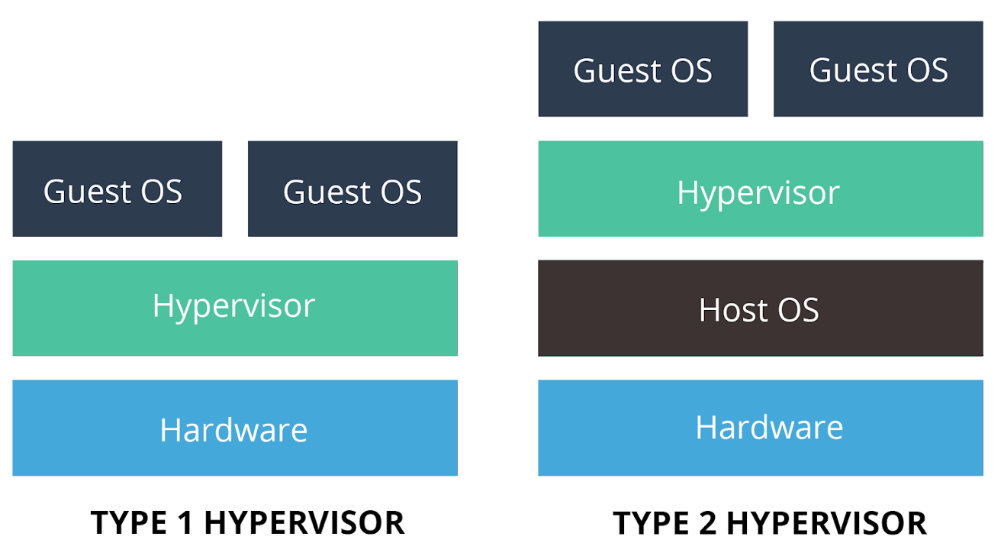
\includegraphics[width=0.6\textwidth]{../imgs/EdA/hipervisor.jpg}
\caption{Tipos de hipervisor}
\label{fig:hipervtypes}
\end{figure}

\subsubsection{VirtualBox}
\subsubsection{VMWare}
\subsection{Virtualización en contenedores}
\subsubsection{LXC}
\subsubsection{Docker}
\section{Tecnologías de aprovisionamiento}
\subsection{Aprovisionamiento estático}
\subsubsection{Docker}
\subsubsection{Vagrant}
\subsection{Aprovisionamiento dinámico}
\subsubsection{Chef}
\subsubsection{Ansible}
\section{Tecnologías de orquestación}
\subsubsection{Docker Compose}
\subsubsection{Kubernetes}
\subsubsection{Terraform}
\subsubsection{A}

	% Desarrollo
\chapter{Desarrollo} \label{ch:des}
\section{} \label{sec:}

	%----------------------------------------------------------------------------------
	% Bibliografía
	\printbibliography[heading=bibintoc]
	%----------------------------------------------------------------------------------
\end{document}
